\noindent

\includegraphics[height=1.25cm]{images/pictograms/replication}

\includegraphics[height=1.25cm]{images/pictograms/benchmark}

\includegraphics[height=1.25cm]{images/pictograms/under_construction}

\includegraphics[height=1.25cm]{images/pictograms/FDM}
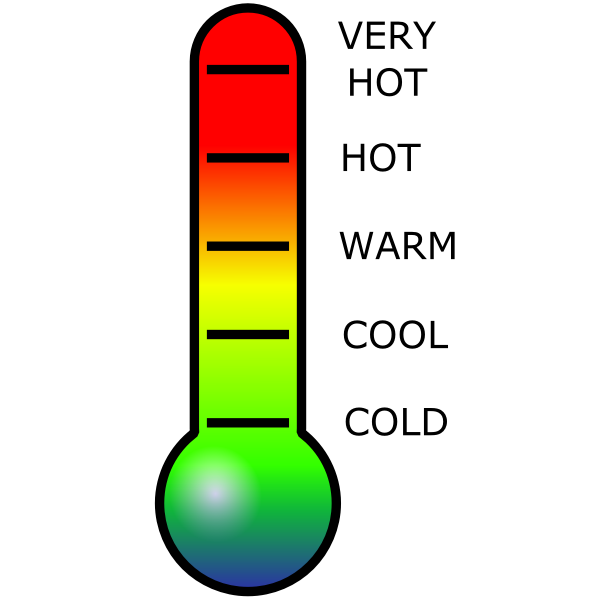
\includegraphics[height=1.25cm]{images/pictograms/temperature}

\includegraphics[height=1.25cm]{images/pictograms/paraview}

%%%%%%%%%%%%%%%%%%%%%%%%%%%%%%%%%%%%%%%%%%%%%%%%%%%%%%%%%%%%%%%%%%%%%%%%%%%%%%%%%%%%%%%%%%%%%%%%%%%

\begin{flushright} {\tiny {\color{gray} python\_codes/fieldstone\_158/text.tex}} \end{flushright}

%\lstinputlisting[language=bash,basicstyle=\small]{python_codes/template_keywords.key}

\par\noindent\rule{\textwidth}{0.4pt}

\begin{center}
\inpython \hspace{.5cm}
{\small Code: \url{https://github.com/cedrict/fieldstone/tree/master/python_codes/fieldstone_158}}
\end{center}

\par\noindent\rule{\textwidth}{0.4pt}


%%%%%%%%%%%%%%%%%%%%%%%%%%%%%%%%%%%%%%%%%%%%%%%%%%%%%%%%%%%%%%%%%%%%%%%%%%%%%%%%%%%%%%%%%%%%%%%%%%%

Before reading any further please read carefully Section~\ref{MMM-FDMSTOKES}. 



%--------------------------------------------------
\subsection*{Implementation}

The domain is $L_x \times L_y$. 
It is discretised in {\python ncellx}$\times${\python ncelly}.
We then define:
\begin{lstlisting}
ncellx=nnx-1
ncelly=nny-1
ncell=ncellx*ncelly
Nb=nnx*nny       # background mesh
Nu=nnx*ncelly    # u-nodes
Nv=ncellx*nny    # v-nodes  
Np=ncellx*ncelly # p-nodes
N=Nu+Nv+Np       # total nb of unknowns
\end{lstlisting}
For the mesh above we have

\begin{verbatim}
nnx= 6
nny= 5
Nb= 30
Nu= 24
Nv= 25
Np= 20
N= 69
ncell= 20
\end{verbatim}


Also, because we will need the cell dimensions and their inverse a lot we define:
\begin{lstlisting}
hx=Lx/(nnx-1)
hy=Ly/(nny-1)
hhx=1/hx
hhy=1/hy
\end{lstlisting}

We must then define the $\delta_{bc}$ parameter that 
controls whether boundaries are free slip or no slip
(see Eq.~\eqref{MMM-eq:XXX}.
We here assigne one $\delta_{bc}$ parameter per side 
of the domain and arbitrarily choose that free slip is 
default:

\begin{lstlisting}
bottom_no_slip=False
top_no_slip=False
left_no_slip=False
right_no_slip=False

if bottom_no_slip:
   delta_bc_bottom=-1
else:
   delta_bc_bottom=+1

if top_no_slip:
   delta_bc_top=-1
else:
   delta_bc_top=+1

if left_no_slip:
   delta_bc_left=-1
else:
   delta_bc_left=+1

if right_no_slip:
   delta_bc_right=-1
else:
   delta_bc_right=+1
\end{lstlisting}



We store the coordinates of the background nodes (where 
density and viscosity live) in arrays {\python xb,yb}, 
$u$ nodes in arrays {\python xu,yu},
the coordinates of the $v$ nodes in arrays {\python xv,yv},
and the coordinates of the $p$ nodes in arrays {\python xp,yp}.

\begin{lstlisting}
xu=np.zeros(Nu,dtype=np.float64)
yu=np.zeros(Nu,dtype=np.float64)
u=np.zeros(Nu,dtype=np.float64)
...
xv=np.zeros(Nv,dtype=np.float64)
yv=np.zeros(Nv,dtype=np.float64)
v=np.zeros(Nv,dtype=np.float64)
...
xp=np.zeros(Np,dtype=np.float64)
yp=np.zeros(Np,dtype=np.float64)
p=np.zeros(Np,dtype=np.float64)
\end{lstlisting}

The code first loops over all $u$-nodes, then all $v$-nodes
and then $p$-nodes. For each node it establishes the index
of all the required stencil neighbouring points.
These are printed when the code is ran in debug mode.
For example we will read:


\begin{multicols}{3}

\begin{verbatim}
u node # 4
ii,jj = 4 0
index_eta_nw= 9
index_eta_n = 10
index_eta_ne= 11
index_eta_sw= 3
index_eta_s = 4
index_eta_se= 5
index_p_w = 3
index_p_e = 4
index_rho_n = 10
index_rho_s = 4
index_v_sw = 3
index_v_se = 4
index_v_nw = 8
index_v_ne = 9
index_u_n = 10
index_u_s = -2
index_u_w = 3
index_u_e = 5
\end{verbatim}
\columnbreak
\begin{verbatim}
v node # 7
ii,jj = 2 1
index_eta_sw= 2
index_eta_w = 8
index_eta_nw= 14
index_eta_se= 3
index_eta_e = 9
index_eta_ne= 15
index_p_s = 2
index_p_n = 7
index_rho_w = 8
index_rho_e = 9
index_v_w = 6
index_v_e = 8
index_v_s = 2
index_v_n = 12
index_u_sw = 2
index_u_se = 3
index_u_nw = 8
index_u_ne = 9
\end{verbatim}
\columnbreak

\begin{verbatim}
p node # 10
ii,jj = 0 2
index_u_w 12
index_u_e 13
index_v_s 10
index_v_n 15
\end{verbatim}

\end{multicols}

This step is crucial because these indices will be used to know
where to add coefficients in the final assembled matrix. 
If any of them is wrong the generated matrix (and therefore linear system)
might not even have a solution. 


We then start from Eqs.~\eqref{eq:fdmstokes1},\eqref{eq:fdmstokes2} and \eqref{eq:fdmstokes3} 
(the modified versions of these equations containing the $\delta_{bc}$ term do not pose
any kind of additional difficulty so we focus on the standard equations only):


\begin{eqnarray}
\left( \frac{\eta_{\tt n}}{h_y^2} \right) {\color{violet} u_{\tt n}} + 
\left( \frac{2\eta_{\tt e}}{h_x^2} \right) {\color{violet} u_{\tt e}} + 
\left( \frac{2\eta_{\tt w}}{h_x^2} \right) {\color{violet} u_{\tt w}} + 
\left( \frac{\eta_{\tt s}}{h_y^2} \right) {\color{violet} u_{\tt s}} + 
\left( -\frac{2\eta_{\tt e}}{h_x^2} -\frac{2\eta_{\tt w}}{h_x^2}  
-\frac{\eta_{\tt n}}{h_y^2} -\frac{\eta_{\tt s}}{h_y^2}  
\right) {\color{violet} u_\otimes} \nn\\
+
\left( \frac{\eta_{\tt n}}{h_x h_y} \right) {\color{orange} v_{\tt ne}}+ 
\left(-\frac{\eta_{\tt n}}{h_x h_y} \right) {\color{orange} v_{\tt nw}}+ 
\left(-\frac{\eta_{\tt s}}{h_x h_y} \right) {\color{orange} v_{\tt se}}+ 
\left( \frac{\eta_{\tt s}}{h_x h_y} \right) {\color{orange} v_{\tt sw}} 
- \frac{1}{h_x} {\color{teal}p_{\tt e}} + \frac{1}{h_x} {\color{teal}p_{\tt w}} 
&=& -\frac{\rho_{\tt n}+\rho_{\tt s}}{2} g_x 
\nn\\
\left( \frac{2\eta_{\tt n}}{h_y^2} \right) {\color{orange} v_{\tt n}} +
\left( \frac{ \eta_{\tt e}}{h_x^2} \right) {\color{orange} v_{\tt e}} +
\left( \frac{ \eta_{\tt w}}{h_x^2} \right) {\color{orange} v_{\tt w}} +
\left( \frac{2\eta_{\tt s}}{h_y^2} \right) {\color{orange} v_{\tt s}} +
\left( 
-\frac{\eta_{\tt e}}{h_x^2} 
-\frac{\eta_{\tt w}}{h_x^2} 
-\frac{2\eta_{\tt n}}{h_y^2} 
-\frac{2\eta_{\tt s}}{h_y^2} 
\right) {\color{orange} v_\otimes} \nn\\
+
\left( \frac{\eta_{\tt e}}{h_x h_y} \right) {\color{violet} u_{\tt ne}} +
\left(-\frac{\eta_{\tt e}}{h_x h_y} \right) {\color{violet} u_{\tt se}} +
\left(-\frac{\eta_{\tt w}}{h_x h_y} \right) {\color{violet} u_{\tt nw}} +
\left( \frac{\eta_{\tt w}}{h_x h_y} \right) {\color{violet} u_{\tt sw}} 
-\frac{1}{h_y} {\color{teal}p_{\tt n}} + \frac{1}{h_y} {\color{teal}p_{\tt s}}
&=& -\frac{\rho_{\tt e}+\rho_{\tt w}}{2} g_y \nn\\
\frac{{\color{violet}u_{\tt e}}-{\color{violet}u_{\tt w}}}{h_x} 
+
\frac{{\color{orange}v_{\tt n}}-{\color{orange}v_{\tt s}}}{h_y} 
&=&0 \nn
\end{eqnarray}



We can define
\begin{align}
\eta_{{\tt n},yy} &= \frac{\eta_{\tt n}}{h_y^2}  &
\eta_{{\tt n},xy} &= \frac{\eta_{\tt n}}{h_xh_y}  \nn\\
\eta_{{\tt s},yy} &= \frac{\eta_{\tt s}}{h_y^2}  &
\eta_{{\tt s},xy} &= \frac{\eta_{\tt s}}{h_xh_y}  \nn\\
\eta_{{\tt e},xx} &= \frac{\eta_{\tt e}}{h_x^2}  &
\eta_{{\tt e},xy} &= \frac{\eta_{\tt e}}{h_xh_y}  \nn\\
\eta_{{\tt w},xx} &= \frac{\eta_{\tt w}}{h_x^2}  &
\eta_{{\tt w},xy} &= \frac{\eta_{\tt w}}{h_xh_y}  \nn\\
\rho_{{\tt ns}}   &= \frac12 (\rho_{\tt n}+\rho_{\tt s}) &
\rho_{{\tt ew}}   &= \frac12 (\rho_{\tt e}+\rho_{\tt w}) \nn\\
\tilde{h}_x &=h_x^{-1} &
\tilde{h}_y &=h_y^{-1} \nn
\end{align}

which translates as follows in the code:

\begin{lstlisting}
eta_n_yy=eta_n/hy**2 ; eta_n_xy=eta_n/hx/hy
eta_e_xx=eta_e/hx**2
eta_w_xx=eta_w/hx**2
eta_s_yy=eta_s/hy**2 ; eta_s_xy=eta_s/hx/hy
...
eta_n_yy=eta_n/hy**2
eta_s_yy=eta_n/hy**2
eta_e_xx=eta_e/hx**2 ; eta_e_xy=eta_e/hx/hy
eta_w_xx=eta_w/hx**2 ; eta_w_xy=eta_w/hx/hy
\end{lstlisting}



so that we can write the three stencil equations as follows:

\begin{eqnarray}
\left( \eta_{{\tt n},yy} \right) {\color{violet} u_{\tt n}} + 
\left( 2\eta_{{\tt e},xx} \right) {\color{violet} u_{\tt e}} + 
\left( 2\eta_{{\tt w},xx} \right) {\color{violet} u_{\tt w}} + 
\left( \eta_{{\tt s},yy} \right) {\color{violet} u_{\tt s}} + 
\left( -2\eta_{{\tt e},xx} - 2\eta_{{\tt w},xx}
-\eta_{{\tt n},yy} -\eta_{{\tt s},yy}
\right) {\color{violet} u_\otimes} \nn\\
+
\left( \eta_{{\tt n},xy} \right) {\color{orange} v_{\tt ne}}+ 
\left(-\eta_{{\tt n},xy} \right) {\color{orange} v_{\tt nw}}+ 
\left(-\eta_{{\tt s},xy} \right) {\color{orange} v_{\tt se}}+ 
\left( \eta_{{\tt s},xy} \right) {\color{orange} v_{\tt sw}} 
+(- \tilde{h}_x) {\color{teal}p_{\tt e}} + (\tilde{h}_x ){\color{teal}p_{\tt w}} 
&=& -\rho_{\tt ns} g_x 
\nn\\
\left( 2\eta_{{\tt n},yy} \right) {\color{orange} v_{\tt n}} +
\left(  \eta_{{\tt e},xx} \right) {\color{orange} v_{\tt e}} +
\left(  \eta_{{\tt w},xx} \right) {\color{orange} v_{\tt w}} +
\left( 2\eta_{{\tt s},yy} \right) {\color{orange} v_{\tt s}} +
\left( 
-\eta_{{\tt e},xx}
-\eta_{{\tt w},xx}
-2\eta_{{\tt n},yy}
-2\eta_{{\tt s},yy}
\right) {\color{orange} v_\otimes} \nn\\
+
\left( \eta_{{\tt e},xy} \right) {\color{violet} u_{\tt ne}} +
\left(-\eta_{{\tt e},xy} \right) {\color{violet} u_{\tt se}} +
\left(-\eta_{{\tt w},xy} \right) {\color{violet} u_{\tt nw}} +
\left( \eta_{{\tt w},xy} \right) {\color{violet} u_{\tt sw}} 
+(-\tilde{h}_y ){\color{teal}p_{\tt n}} + (\tilde{h}_y) {\color{teal}p_{\tt s}}
&=& -\rho_{\tt ew} g_y \nn\\
(\tilde{h}_x) {\color{violet}u_{\tt e}}- 
(\tilde{h}_x) {\color{violet}u_{\tt w}}
+
(\tilde{h}_y) {\color{orange}v_{\tt n}}- 
(\tilde{h}_y){\color{orange}v_{\tt s}} &=&0 \nn
\end{eqnarray}



Let us now create the vector $\vec{X}$ that is $N=N_u+N_v+N_p=43$ long (still considering 
the $4\times 3$ cell mesh presented above):
\[
\vec{X}^T=(
u_{\tt \color{violet} 0},u_{\tt \color{violet} 1}, \dots , u_{\tt \color{violet} 14},
v_{\tt \color{orange} 0},v_{\tt \color{orange} 1}, \dots , v_{\tt \color{orange} 15},
p_{\tt \color{teal} 0},p_{\tt \color{teal} 1}, \dots, p_{\tt \color{teal} 11})
\]
We have 14 boundary conditions and 29 stencil equations that establish relationships between 
unknowns  (see previous section) which we can write altogether as a linear system.

The boundary condition $u_{\color{violet} \tt 0}=0$ can be written 
\[
(1,0,0,0,...,0) \cdot \vec{X} = (0,....)^T
\]
so that the lhs horizontal vector becomes the first line of the matrix and we
must write zero in the first element of the rhs vector. 

Likewise the boundary condition $u_{\color{violet} \tt 4}=0$ can be written
\[
(0,0,0,0,1,...,0) \cdot \vec{X} = (.,.,.,.,0,....)^T
\]
and the lhs horizontal vector becomes the 5th line of the matrix and we
must write zero in the 5th element of the rhs vector. 

We repeat this procedure for all $u$ boundary conditions, which allows us to fill 
the 1st, 5th, 6th, 10th, 11th and 14th line of the matrix.

Likewise the boundary conditions on $v$ will yield similar lines in the matrix, 
only the corresponding lines are below the 15 first ones corresponding to $u$.

Considering node ${\color{violet} u_7}$, the stencil equation \eqref{eq:fdmstokes1} then becomes:



\begin{eqnarray}
\left( \frac{\eta_{\tt n}}{h_y^2} \right) {\color{violet} u_{\tt 12}} + 
\left( \frac{2\eta_{\tt e}}{h_x^2} \right) {\color{violet} u_{\tt 8}} + 
\left( \frac{2\eta_{\tt w}}{h_x^2} \right) {\color{violet} u_{\tt 6}} + 
\left( \frac{\eta_{\tt s}}{h_y^2} \right) {\color{violet} u_{\tt 2}} + 
\left( -\frac{2\eta_{\tt e}}{h_x^2} -\frac{2\eta_{\tt w}}{h_x^2}  
-\frac{\eta_{\tt n}}{h_y^2} -\frac{\eta_{\tt s}}{h_y^2}  
\right) {\color{violet} u_7} \nn\\
+
\left( \frac{\eta_{\tt n}}{h_x h_y} \right) {\color{orange} v_{\tt 10}}+ 
\left(-\frac{\eta_{\tt n}}{h_x h_y} \right) {\color{orange} v_{\tt 9}}+ 
\left(-\frac{\eta_{\tt s}}{h_x h_y} \right) {\color{orange} v_{\tt 6}}+ 
\left( \frac{\eta_{\tt s}}{h_x h_y} \right) {\color{orange} v_{\tt 5}} 
- \frac{1}{h_x} {\color{teal}p_{\tt 6}} + \frac{1}{h_x} {\color{teal}p_{\tt 5}} 
&=& -\frac{\rho_{\tt 12}+\rho_{\tt 7}}{2} g_x \nn
\end{eqnarray}
which will correspond to the 7th line in the matrix. The coefficients inside the 
parentheses will be input in the column corresponding to the unknowns they front. 



Because of how the $\vec{X}$ vector is built (first ${\color{violet} u}$, 
then ${\color{orange}v}$ then ${\color{teal} p}$ unknowns)
the resulting linear system takes the following form:
\begin{equation}
\left(
\begin{array}{ccc}
\K_{xx} & \K_{xy} & \G_x \\
\K_{yx} & \K_{yy} & \G_y \\
\Q_x & \Q_y & 0
\end{array}
\right)
\cdot
\vec{X}
=\vec{b}
\label{eq:fdmstokes6}
\end{equation}


\newpage
The logic of the code with regards to matrix and rhs assembly is as follows:

\begin{lstlisting}
###########################################################
# loop over all u nodes
###########################################################
for i in range(0,Nu):
    if left[i]: # u node on left boundary
       A[...,...]=...
       b[...]=...
    elif right[i]: # u node on right boundary
       A[...,...]=...
       b[...]=...
    else:
       ...
       if jj==0: # bottom row, ghosts nodes used
          A[...,...]=...
          b[...]=...
       elif jj==ncelly-1: # top row, ghosts nodes used
          A[...,...]=...
          b[...]=...
       else:
          A[...,...]=...
          b[...]=...

###########################################################
# loop over all v nodes
###########################################################
for i in range(0,Nv):
    if bottom[i]: # v node on bottom boundary
       A[...,...]=...
       b[...]=...
    elif top[i]: # v node on top boundary
       A[...,...]=...
       b[...]=...
    else:
       if ii==0: # left column, ghosts nodes used
          A[...,...]=...
          b[...]=...
       elif ii==ncellx-1: # right column, ghosts nodes used
          A[...,...]=...
          b[...]=...
       else:
          A[...,...]=...
          b[...]=...

###########################################################
# loop over all p nodes
###########################################################
for i in range(0,Np):
    A[...,...]=...
    b[...]=...
\end{lstlisting}

\newpage

After the loop on $u$ nodes, the first $N_u$ lines have been filled and the matrix non-zero pattern is as follows:
\begin{center}
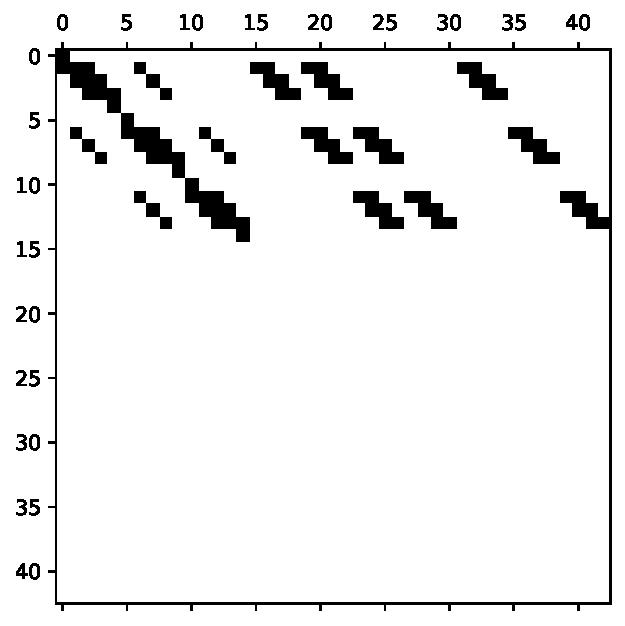
\includegraphics[width=6cm]{python_codes/fieldstone_158/images/matrix_u.pdf}
\end{center}


After the loop on $v$ nodes, the matrix non-zero pattern is as follows:
\begin{center}
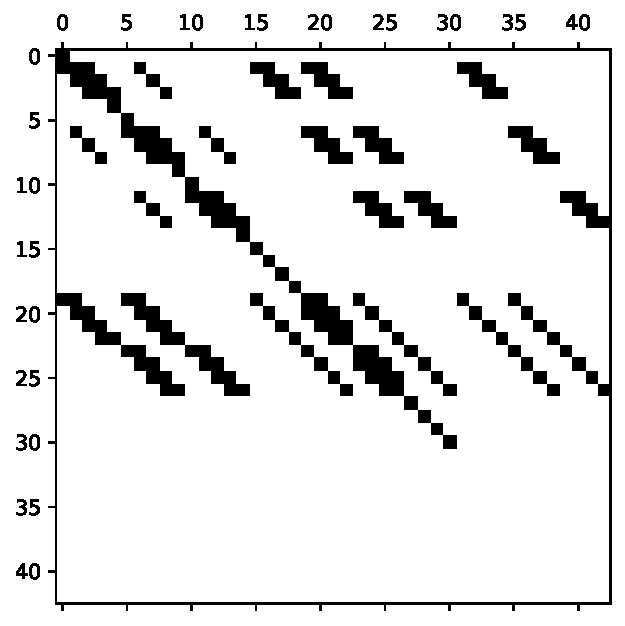
\includegraphics[width=6cm]{python_codes/fieldstone_158/images/matrix_uv.pdf}
\end{center}

And finally after the loop of cells:
\begin{center}
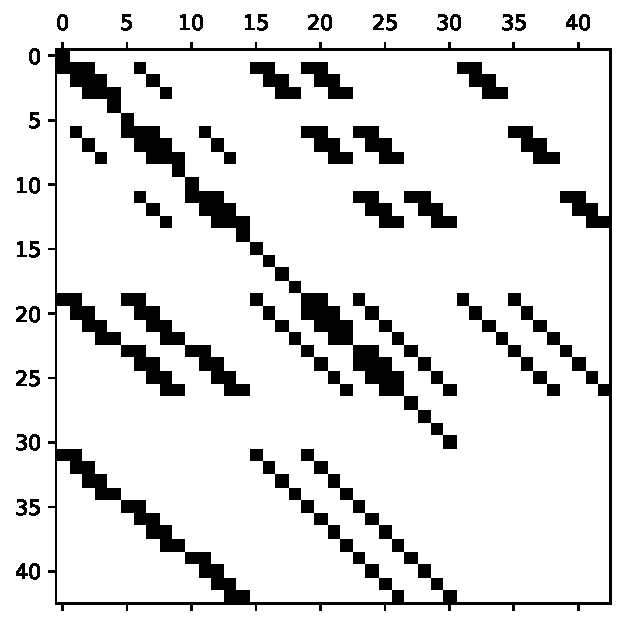
\includegraphics[width=6cm]{python_codes/fieldstone_158/images/matrix_uvp.pdf}
\end{center}
As predicted in Eq.~\eqref{eq:fdmstokes6} we recover a matrix that 
is composed of 8 blocks.




%---------------------------
\subsection*{Experiment 1}

This is a basic sanity check. Boundary conditions are either free slip or no slip.
The domain is the unit square filled with a Newtonian fluid characterised by 
$\rho=1$ and $\eta=1$. There is a sphere in the middle of radius 0.15 with $\rho=2$
and $\eta=10$.

\begin{center}
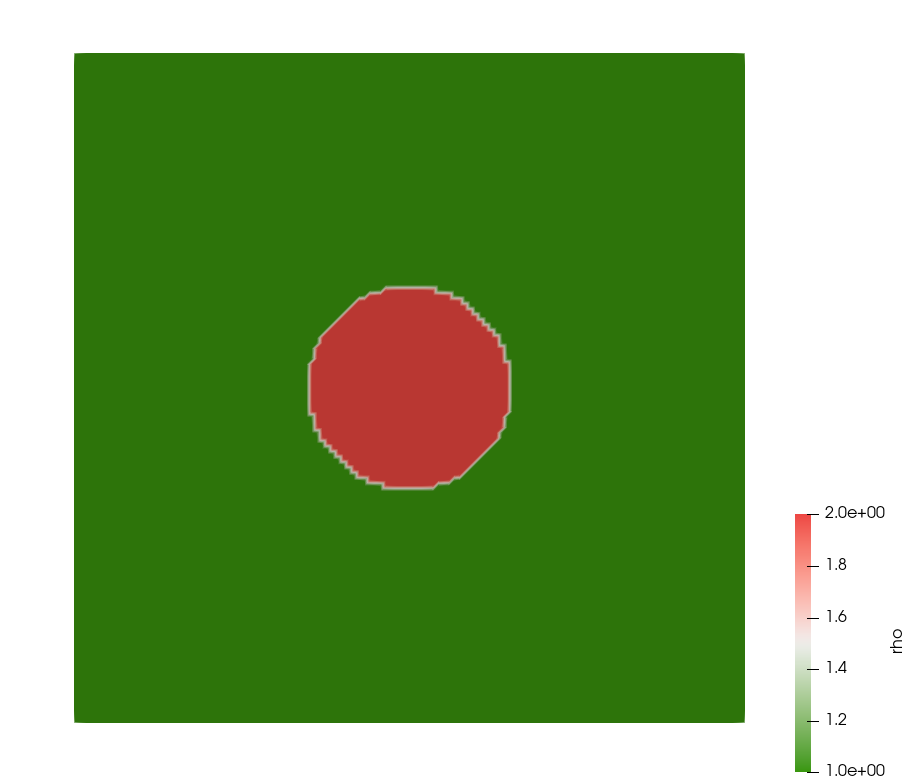
\includegraphics[width=4cm]{python_codes/fieldstone_158/results/exp1/rho}
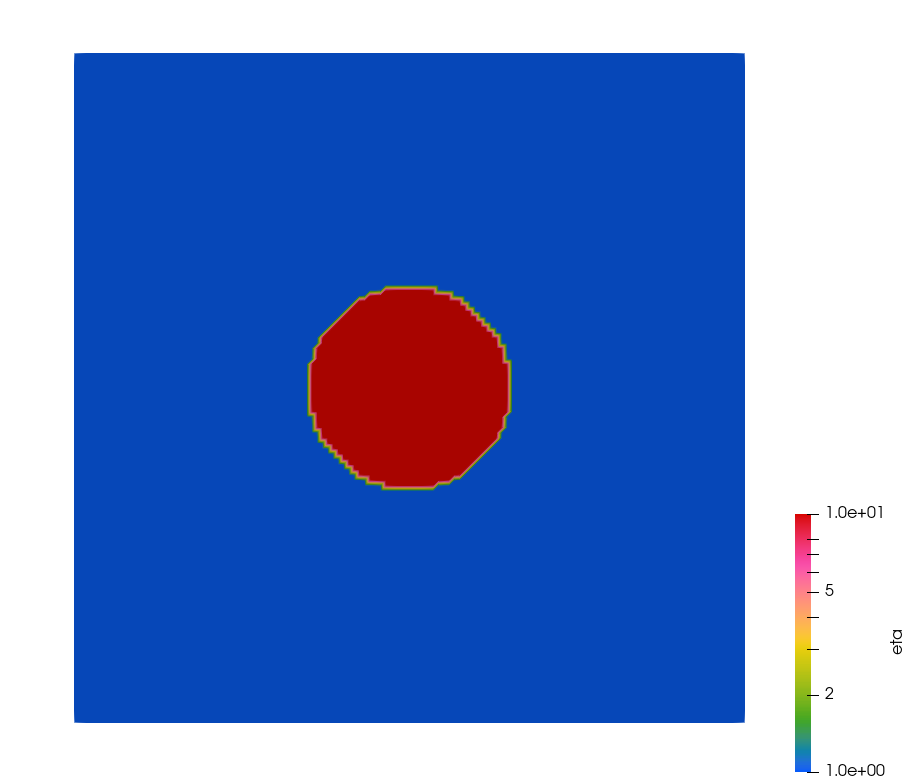
\includegraphics[width=4cm]{python_codes/fieldstone_158/results/exp1/eta}
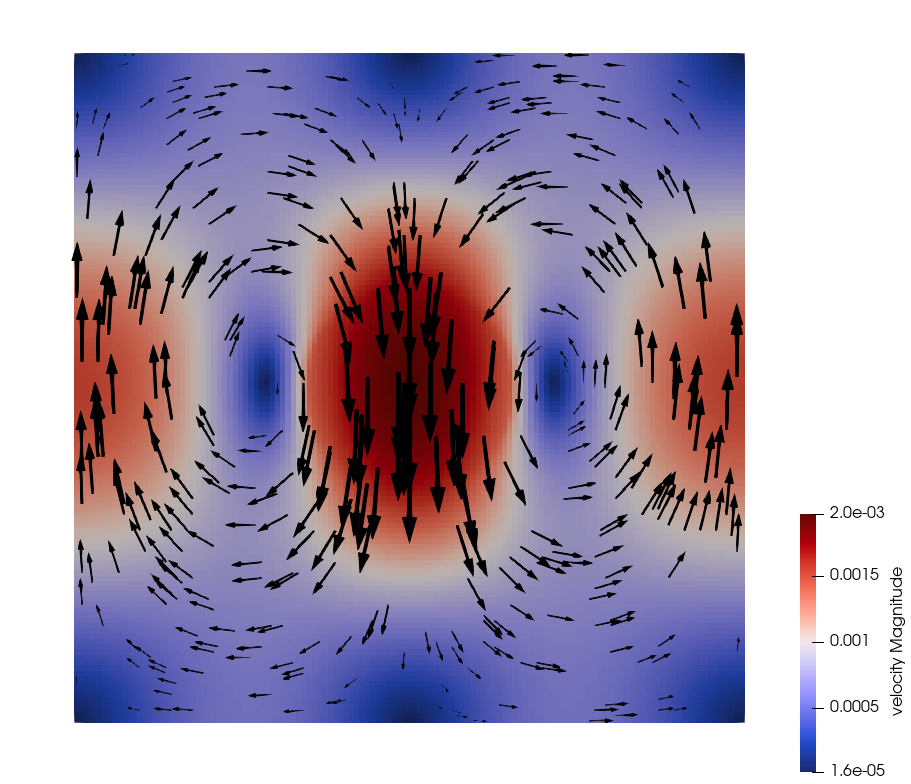
\includegraphics[width=4cm]{python_codes/fieldstone_158/results/exp1/vel}
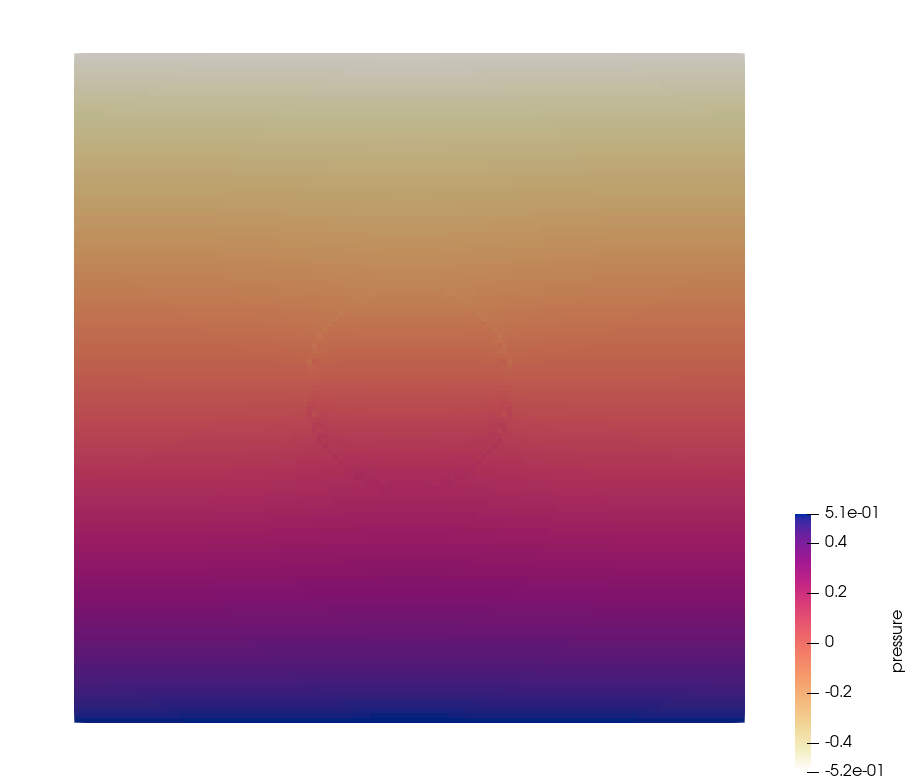
\includegraphics[width=4cm]{python_codes/fieldstone_158/results/exp1/press}
\end{center} 


TODO: compute strain rate

TODO: show free slip vs no slip

TODO: do donea huerta bench




